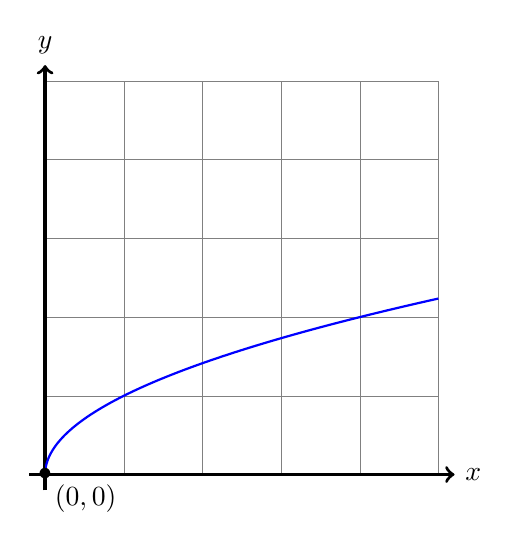
\begin{tikzpicture}
  \draw[very thin,color=gray] (0,0) grid (5,5);

  \draw[very thick,->] (-.2,0) -- (5.2,0) node[right] {$x$};
  \draw[very thick,->] (0,-0.2) -- (0,5.2) node[above] {$y$};

  \begin{scope}[domain=0:5]
    \clip (0,0) rectangle (5,5);
    \draw [color=blue,thick] plot[smooth,samples=500] (\x,{sqrt(\x)});
  \end{scope}

  \node at (0,0) {$\bullet$};
  \node [below right] at (0,0) {$(0,0)$};
\end{tikzpicture}
